\chapter{Source Code}
The source code for the various applications in context of this thesis is found at following Github repository: \textit{https://github.com/perelan/master}

\section{File and Folder Structure}
\begin{description}
    \item[Nidra] encompasses the implementation performed in the Chapther 5. The application follows the MVVM architecture pattern, thus the naming scheme of the folders advertently follows the seperation of the components in the architecture pattern. The folder structure for the application code is seperated into:
    \begin{itemize}
        \item \textbf{Dispatcher}: contains the code for communication with the DataStreamDispatchingModule including the service for data acquisition, and the code for reconnectivity with the sensor sources on sensor disconnect or human disruption.
        \item \textbf{Model}: contains the model for data entities, structure for the sensor data and Flow payload data, and the interface for establishing connection with SQLite (with Android Room).
        \item \textbf{Utils}: comprise of miscellaneous code ranging from functionality to extract Flow payload to logic behind the export functionality. 
        \item \textbf{View}: include the activities (discussed in Chapther 5) with seperation of various views (e.g., feed, module and recording). 
        \item \textbf{ViewModel}: exposes the operations that can be performed on the data entities. 
    \end{itemize}

    \item[DataStreamDispatchingModule] encompasses the implemention made by Bugasjki. However, the application was extended during the course of this thesis and can be reflected into the following files: 
    \begin{itemize}
        \item \textbf{SensorDiscovery} listens for broadcasts sent by the sensor wrappers on start. The data passed alongside the broadcasts is extracted of name and packagename, and stored in a \verb|SharedPreferences| if it does not exists. 
        \item \textbf{Sensor} is the sensor objective that is stored into the \verb|SharedPreferences| mentioned above, with the name and the packagename of the sensor wrapper. 
    \end{itemize}

    \item[Flow] encompasses the driver for creating a sensor wrapper made by Gjøby. The sensor wrapper adds the support for Flow sensor, and the extention made to enable the sensor wrapper (besides the components introduced by Gjøby) are the following:
    \begin{itemize}
        \item \textbf{Bluetooth} include the code for connecting with the Flow sensor with Bluetooth LE. Most of the logic is in the file \verb|BluetoothHandler|, and the code is inspired by the application \textit{RawDataMonitor} sent to us from Sagar Sen at SweetZpot Inc. 
        \item \textbf{View} contains the activity for listing the available sensors on the screen. 
    \end{itemize}

    \item[TestModule] encompasses a boilerplate code for creating a new module (further discussed in Appendix C).
    \item[Thesis] encompasses the LaTeX for this thesis, including figures and UiO master's thesis format.
    \item[Graph] encompasses the data acquired from the various mobile devices during the two concert dates including a Python script for plotting it in a time-series graph.

\end{description}

\chapter{Expatiate on Concert Experiement}

\section{Concert Day 1: Time-Series Graph}
This Section illustrates the samples collected during the concert the concert on third April of 2019, which lasted 
for one hour. There are six individual records for this day: 

\begin{figure}
    \centering
    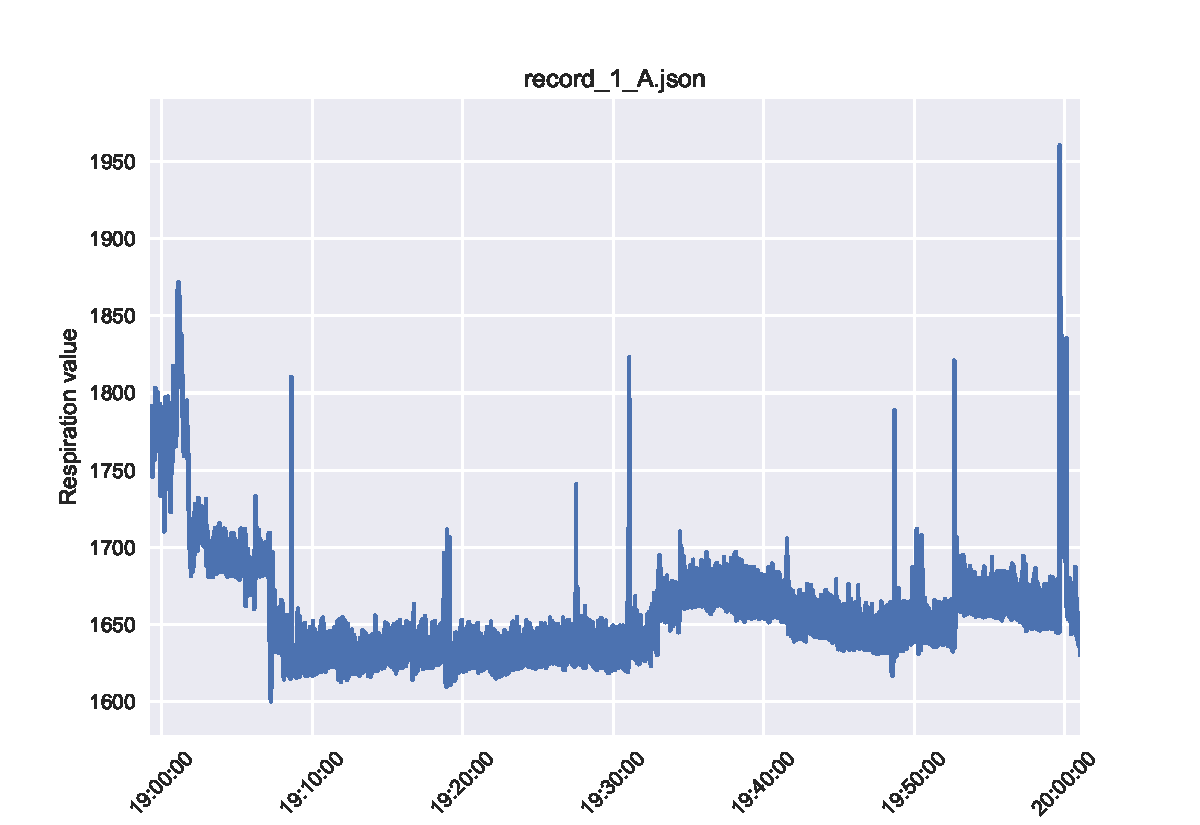
\includegraphics[scale=0.6]{images/record_1_a.pdf}
    \caption{Concert Day 1: Device Model A.}
    \label{fig:concert_day1_a}
\end{figure}

\begin{figure}
    \centering
    \includegraphics[scale=0.6]{images/record_1_b.pdf}
    \caption{Concert Day 1: Device Model B.}
    \label{fig:concert_day1_b}
\end{figure}

\begin{figure}
    \centering
    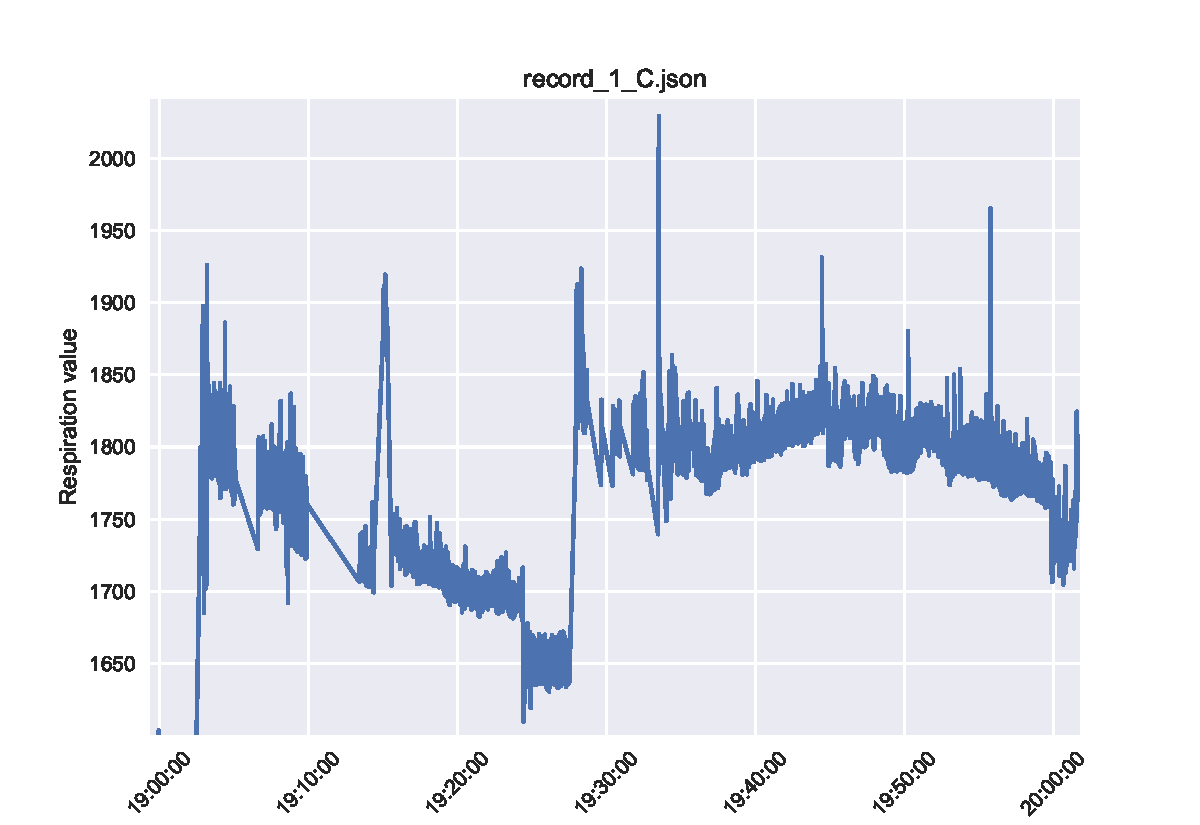
\includegraphics[scale=0.6]{images/record_1_c.pdf}
    \caption{Concert Day 1: Device Model C.}
    \label{fig:concert_day1_c}
\end{figure}

\begin{figure}
    \centering
    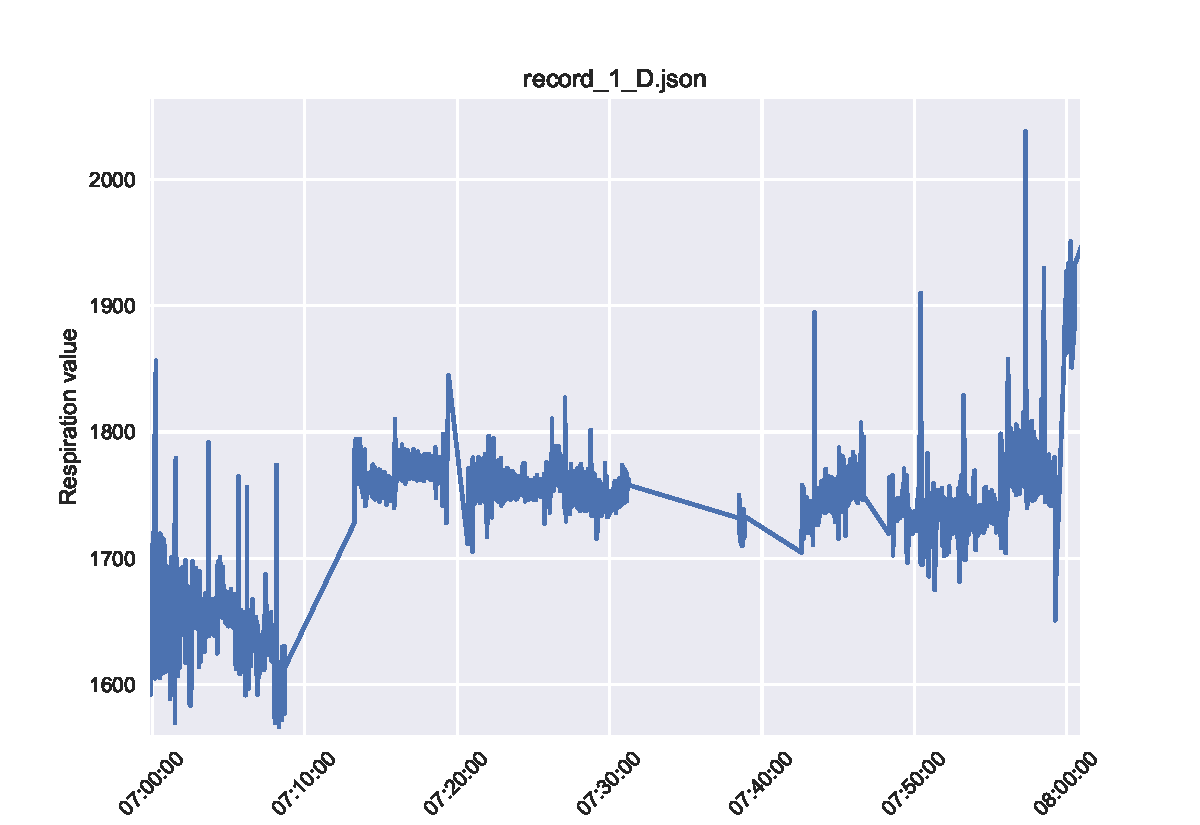
\includegraphics[scale=0.6]{images/record_1_d.pdf}
    \caption{Concert Day 1: Device Model D.}
    \label{fig:concert_day1_d}
\end{figure}

\begin{figure}
    \centering
    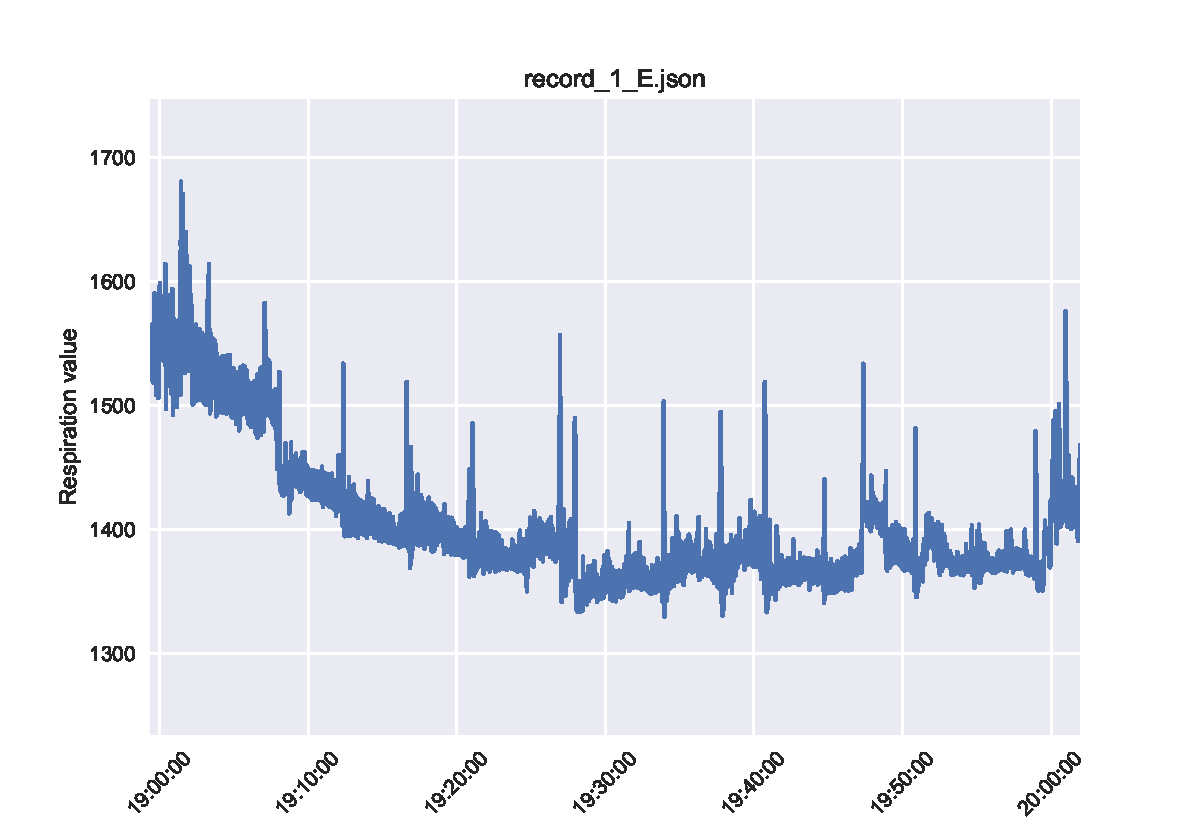
\includegraphics[scale=0.6]{images/record_1_e.pdf}
    \caption{Concert Day 1: Device Model E.}
    \label{fig:concert_day1_e}
\end{figure}

\begin{figure}
    \centering
    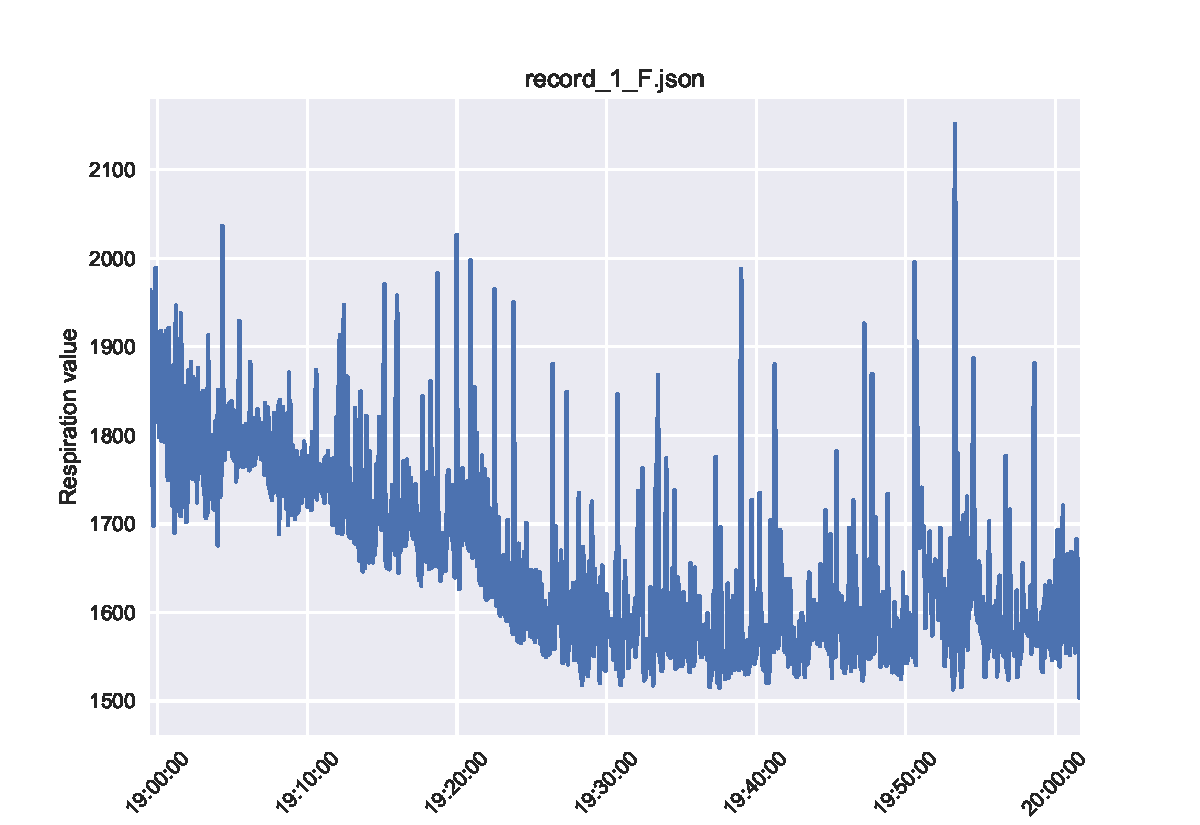
\includegraphics[scale=0.6]{images/record_1_f.pdf}
    \caption{Concert Day 1: Device Model F.}
    \label{fig:concert_day1_f}
\end{figure}

\section{Concert Day 2: Time-Series Graph}


\begin{figure}
    \centering
    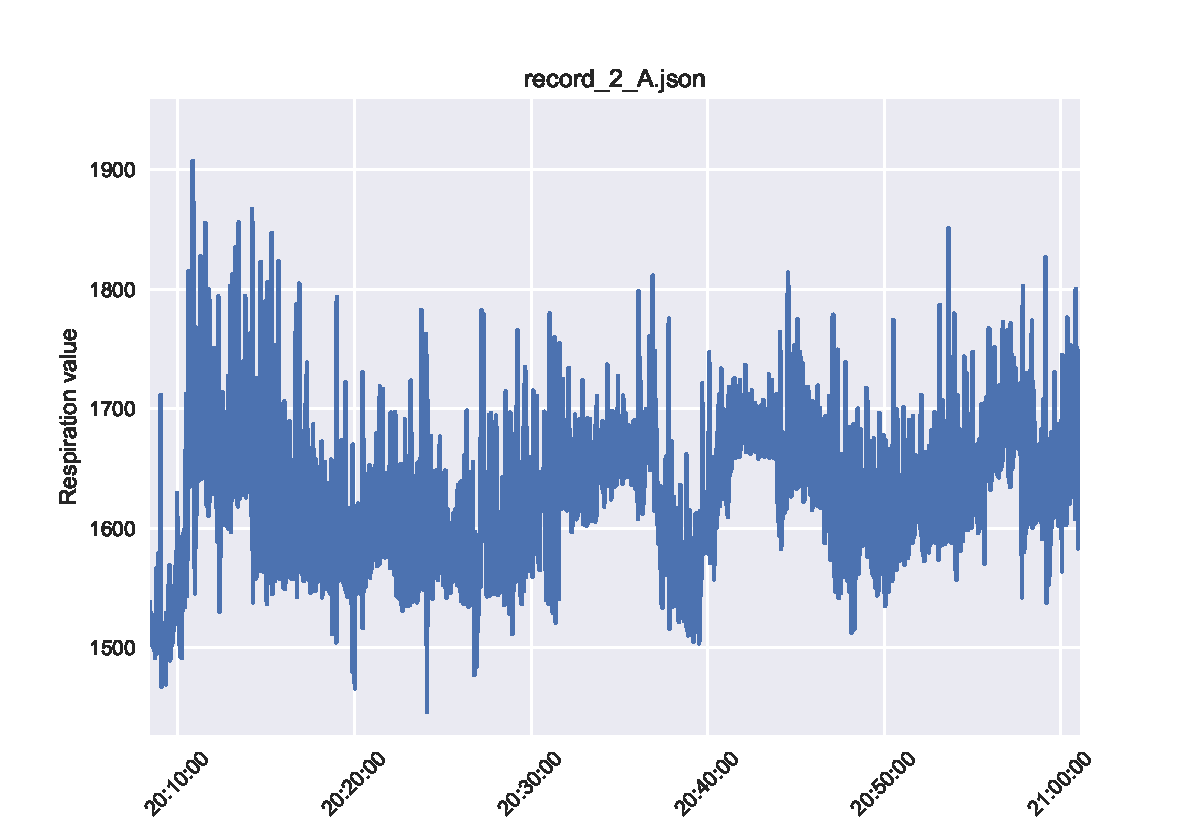
\includegraphics[scale=0.6]{images/record_2_a.pdf}
    \caption{Concert Day 2: Device Model A.}
    \label{fig:concert_day2_a}
\end{figure}

\begin{figure}
    \centering
    \includegraphics[scale=0.6]{images/record_2_b.pdf}
    \caption{Concert Day 2: Device Model B.}
    \label{fig:concert_day2_b}
\end{figure}

\begin{figure}
    \centering
    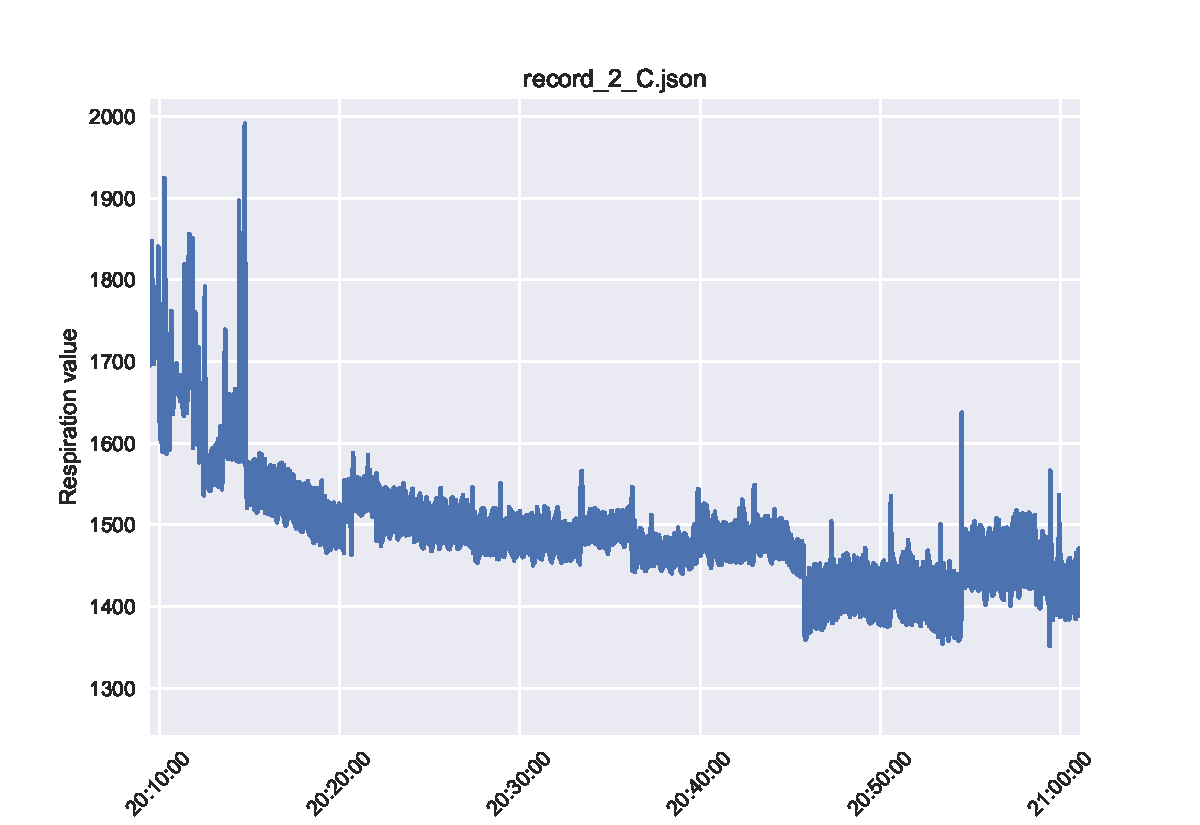
\includegraphics[scale=0.6]{images/record_2_c.pdf}
    \caption{Concert Day 2: Device Model C.}
    \label{fig:concert_day2_c}
\end{figure}

\begin{figure}
    \centering
    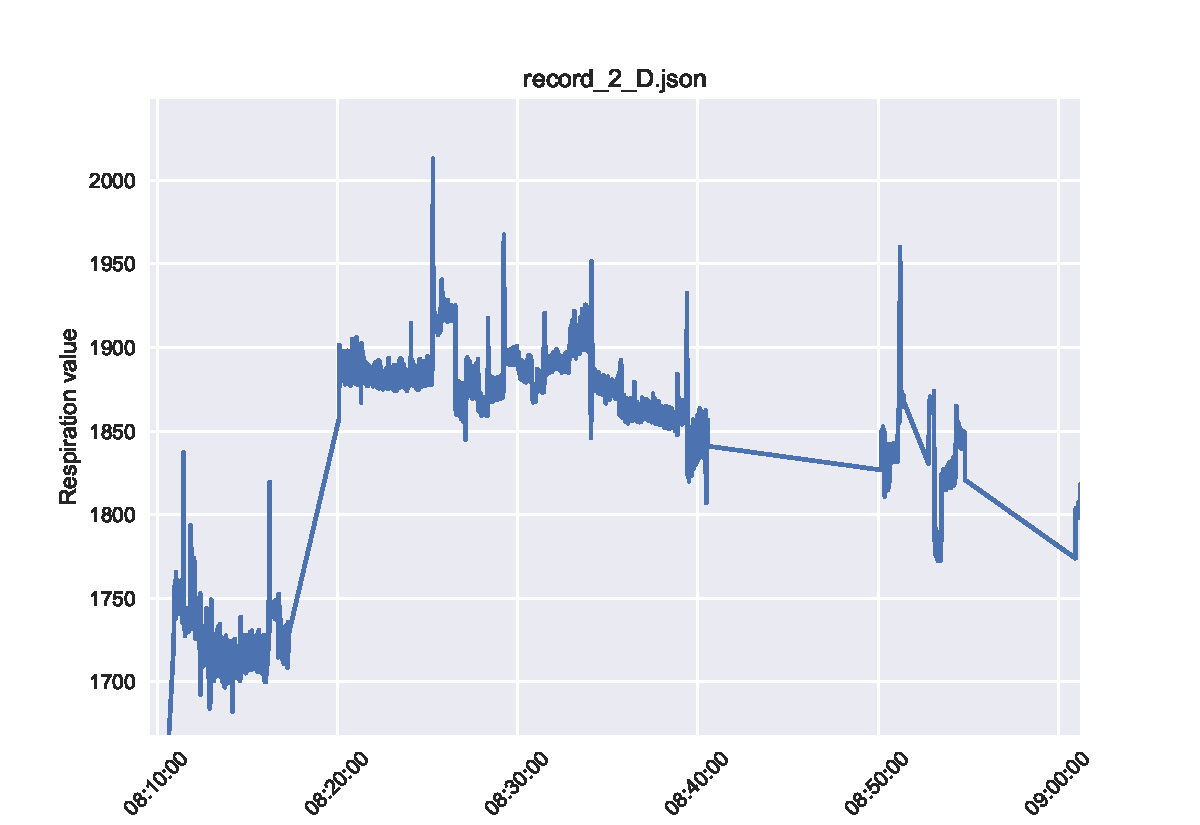
\includegraphics[scale=0.6]{images/record_2_d.pdf}
    \caption{Concert Day 2: Device Model D.}
    \label{fig:concert_day2_d}
\end{figure}

\begin{figure}
    \centering
    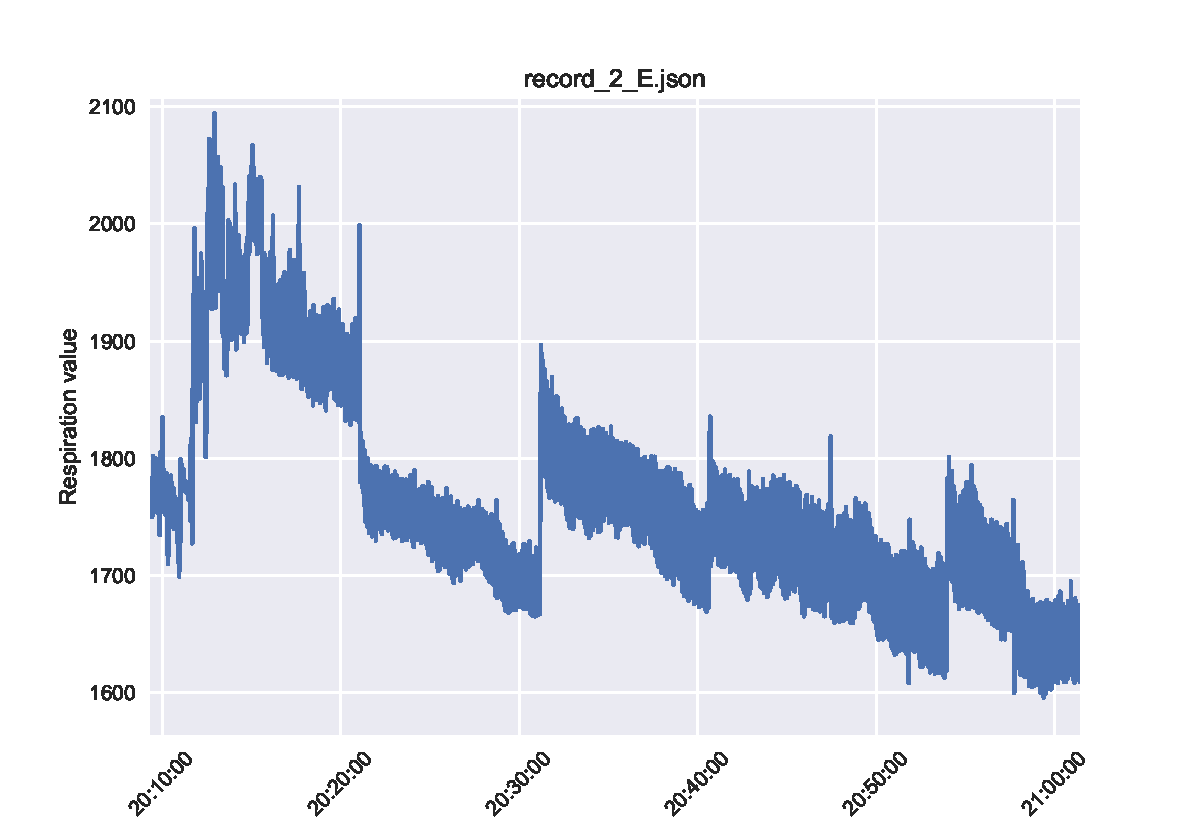
\includegraphics[scale=0.6]{images/record_2_e.pdf}
    \caption{Concert Day 2: Device Model E.}
    \label{fig:concert_day2_e}
\end{figure}

\begin{figure}
    \centering
    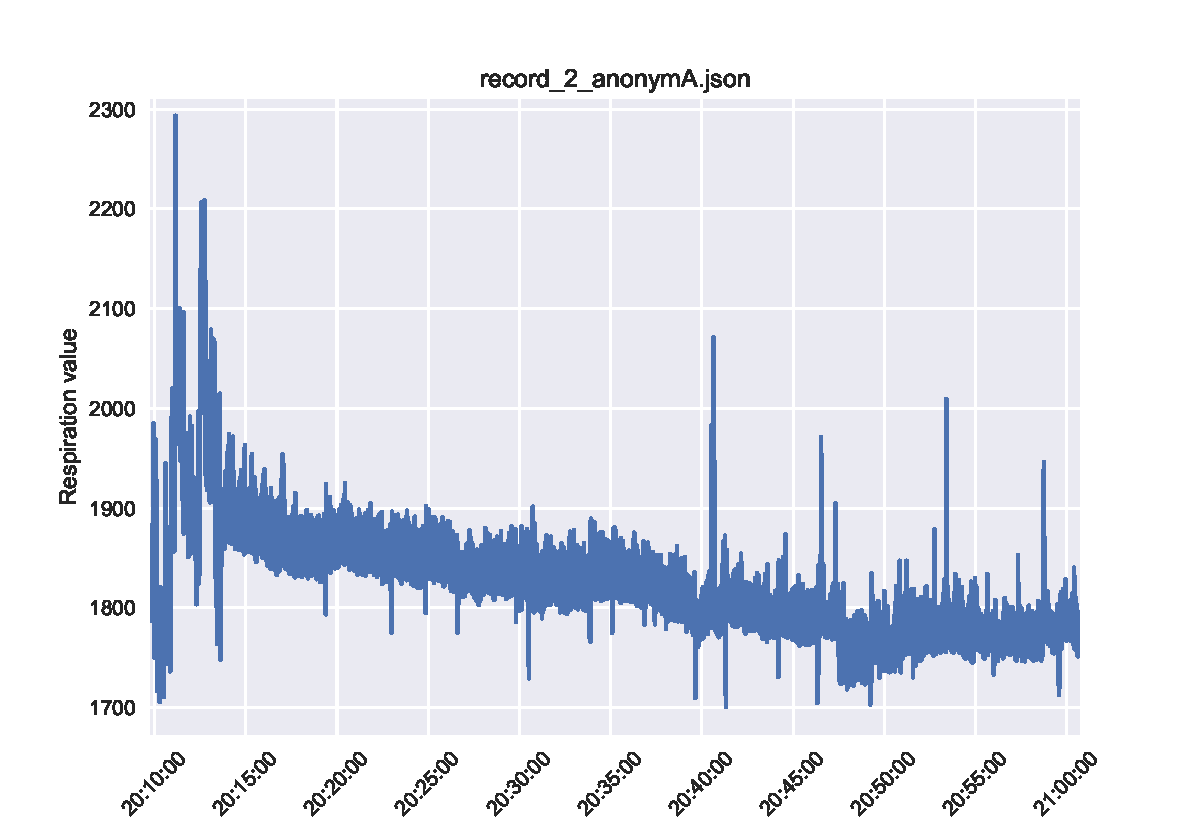
\includegraphics[scale=0.6]{images/record_2_f.pdf}
    \caption{Concert Day 2: Device Model F.}
    \label{fig:concert_day2_f}
\end{figure}

\newpage
\section{Python Code for Plotting}
The following listing presents the code used for plotting the data from the concert into a time-series graph. 

\begin{lstlisting}[language=json, caption={}, captionpos=b]
import json
import matplotlib.pyplot as plt
from matplotlib.dates import DateFormatter
from datetime import datetime
from statistics import mean
import sys 
import seaborn

plt.style.use('seaborn')

sample_count = 0

def get_data(sample):
    data = sample[2].split("=")[1].split(",")
    avg = mean([int(i) for i in data])
    return avg

def get_date(sample):
    global sample_count

    if sample > '20:10:00' and sample < '21:00:00':
        sample_count += 1

    return datetime.strptime(sample, '%H:%M:%S')

def parse(data, name):
    global sample_count

    date = [get_date(i['implicitTS'].split(" ")[-1]) for i in data[0]['samples']]
    data = [get_data(i['sample'].split(", ")) for i in data[0]['samples']]

    fig, ax = plt.subplots()
    plt.plot(date, data)

    ax.xaxis.set_major_formatter(DateFormatter('%H:%M:%S'))
    ax.xaxis_date()
    ax.xaxis.set_tick_params(rotation=45)

    ax.set_xlabel("Time")
    ax.set_ylabel("Respiration value")
    ax.set_title(name)

    plt.show()
    
    print(sample_count)

def read(filename="record_1_B.json"):
    with open(filename) as f:
        json_data = json.load(f)

        parse(json_data, filename)

if __name__ == "__main__":
    if len(sys.argv) == 2:
        read(sys.argv[1])
    else:
        read()
\end{lstlisting}


\chapter{Module Template}
To expedite the creation of a new module a template with pre-code is provided. The pre-code contains a blank Android project with the latest Gradle version 3.4.0 and support for Android 9 (API level 28). In the subsequent Sections, the instructions of duplicating the template is presented. 



\section{Application Setup}

\subsection{Download the Application}
Start by locating the \textit{ModuleTemplate} application in the Github repository for this thesis. Download the application folder, rename it with desired name, and move it to the \verb|Android Studio| project folder. The listing below presents the commands to accomidate for the actions. Next, import the project in Android Studio by pressing \verb|File --> Open --> (Name of Application)|

\begin{lstlisting}[language=json, caption={}, captionpos=b]
git clone https://github.com/Perelan/Master.git
cd Master
mv ModuleTemplate <Path to Android Studio Project>/<Desired Name>
\end{lstlisting}

\subsection{Change the Name of the Application}
Change the name of the application such that the user can locate the application in the app drawer, also the name is used as the module-name when listed in Nidra. The name change is performed by locating the \verb|app_name| inside of \verb|strings.xml| which is to be found in \verb|res/value|, see Listing below. 

\begin{lstlisting}[language=json, caption={}, captionpos=b]
<resources>
    <string name="app_name">ModuleTemplate</string> <-- Change this!
</resources>
\end{lstlisting}

\subsection{Rename the Package of the Application}
Change the package name of the application by following the listing below. It is incentivized to keep the prefix of \textit{com.cesar.X} to group future modules by the package name. 

\begin{lstlisting}[language=json, caption={}, captionpos=b]
Right Click => Refactor => Rename => Rename Package => *new package name* => Refactor
\end{lstlisting}

\subsection{Change the Application ID}
Finally, change the application ID respectivly to the package name defined above---the ID is used to seperate installed applications from each other. The application ID is located in the \verb|build.gradle| file inside of the \verb|app| folder of the project. See the listing below.

\begin{lstlisting}[language=json, caption={}, captionpos=b]
android {
    defaultConfig {
        applicationId "com.cesar.moduletemplate"
    }
}
\end{lstlisting}

\section{Application Execution}


\subsection{Add the Module to Nidra}
In order to retrieve the records data, the module-application has to be added to Nidra. Therefore, launch the Nidra application on the device and navigate to the modules screen. Press the \textit{Add new Module} button, find the module by name in the list and click to add. 

\subsection{Retrieve the Data}
The data is sent as a JSON string to the module when it is launched within Nidra. The pre-code is seperated into following files and folder:

\begin{description}
    \item[MainActivity] On creation of the module-application, the bundle of data that is sent as an Intent is passed to the \verb|Extract| method in \verb|DataExtraction|.
    \item[DataExtraction] The \verb|Extract| method retrieves the JSON string from the bundle with the key \textit{data}, and returns a unmarshalls of the data into a \verb|PayloadFormat| object
    \item[Payload/PayloadFormat] Is the object in which one of the record with corresponding samples of the data is marshalled. It encompasses a single record that contains metadata and user information, also a list of samples. 
    \item[Payload/Record] contains the record metadata (see Section \ref{des:dataentity})
    \item[Payload/Sample] contains a single sample (see Section \ref{des:dataentity})
    \item[Payload/User] contains the state of the user information at the given time of recording (see Section \ref{des:dataentity}).
\end{description}

As part of the discussion of the module design, the records is sent to the module-application only when it is launched within Nidra. This might become cumbersome in the long run, therefore, it is highly incentivized to temporarly cache the data under development. 


\chapter{Flow Sensor Wrapper}

\begin{figure}[!h]
    \centering
    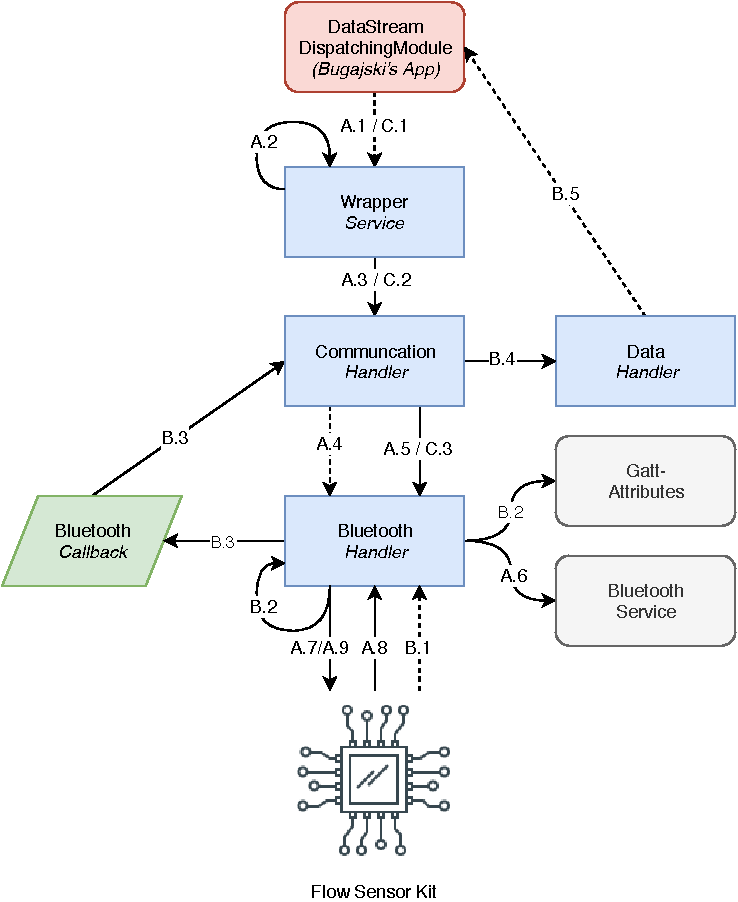
\includegraphics[scale=0.7]{images/Flow_Imp.pdf}
    \caption{Implementation of Flow sensor wrapper.}
    \label{fig:impl_flowsensor}
\end{figure}

A description of flow sensor wrapper is described in Section \ref{imp:flowsensor}. The following sections describes the functionality of the sensor wrapper by separating them into following actions: (A) starting the data acquisition; (B) handle the samples from the sensor; and (C) stopping the data acquistion. The flow for the actions is presented in Figure \ref{fig:impl_flowsensor}.

\section{Implementation}


\subsection{Action A: Starting the Data Acquistion}
Action A is to start the data acquestion based on the command sent by 

\begin{itemize}
    \item[A.1] A broadcast from the DSDM with a Intent of \textit{Start} is sent to the \verb|WrapperService|.
    \item[A.2] Within the \verb|WrapperService|, a binder between the between this service component and the DSDM is created (which will be used for sending data by the Flow sensor). Moreover, a new thread for the \verb|CommuncationHandler| is created and started.
    \item[A.3] This component initalizes the connectivity with the \verb|BluetoothHandler| service, and listens for data packets from that component.
    \item[A.4] A reference to the \verb|BlueToothHandler| with a binder is created, in order to communicate with the service. 
    \item[A.5] Moreover, the request to connect and start the acquesition is sent to the \verb|BluetoothHandler|. 
    \item[A.6] \verb|BluetootHandler| creates an object of the \verb|BluetoothHandler|, which contains the state of the sensor source (e.g., battery level, breathing data enabled, and manufacturer name). 
    \item[A.7] The \verb|BluetootHandler| connects with the GATT server (the Flow sensor), and once the connectivity is established (using the Android provided API's for connecting with the Bluetooth LE devices), we can ask the sensor source for available services. 
    \item[A.8] The sensor source responds with all of the avaiable services and characterstics, and we can proceed to notify the sensor source to enable the breathing data and the battery level service.  
\end{itemize}


\subsection{Action B: Handle the Samples from the Sensor}

\begin{itemize}
    \item[B.1] Peridocally, the Flow sensor sends data to the connected mobile device, based on the activated service (i.e., breathing data and battery level). These samples are sent to the connectivity established earlier. 
    \item[B.2]  The BlueToothHandler handles these data packets (by filtering them out on GattAttributes) and reads the value from the characterstics that is encompassed in the service.
    \item[B.3] The values are sent as a callback to the \verb|CommunicationHandler|. 
    \item[B.4] Which further sends it to the \verb|DataHandler|.
    \item[B.5] The \verb|DataHandler| creates a JSON string that contains meta-data (e.g., the ID of the sensor wrapper) together with the data, and sends the data to the DSDM for further processing.    
\end{itemize}


\subsection{Action C: Stopping the Data Acquestion}

\begin{itemize}
    \item[C.1] A broadcast from the DSDM with a Intent of \textit{Stop} is sent to the \verb|WrapperService|. The \verb|WrapperService| disconnect with the binder that was created between this component service and DSDM. As a result, the \verb|CommunicationHandler| thread is interrupted.
    \item[C.2] The \verb|CommunicationHandler| notifies the \verb|BluetootHandler| to disconnect with the GATT server and terminate.
    \item[C.3] The \verb|BluetootHandler| disconnects the connectivity with the Flow sensor wrapper, and further notifies the components that the communication is closed (e.g., the main screen can change the state displaying that it is connected to disconnected) 
\end{itemize}



\section{Presentation}
\begin{figure}
    \centering
    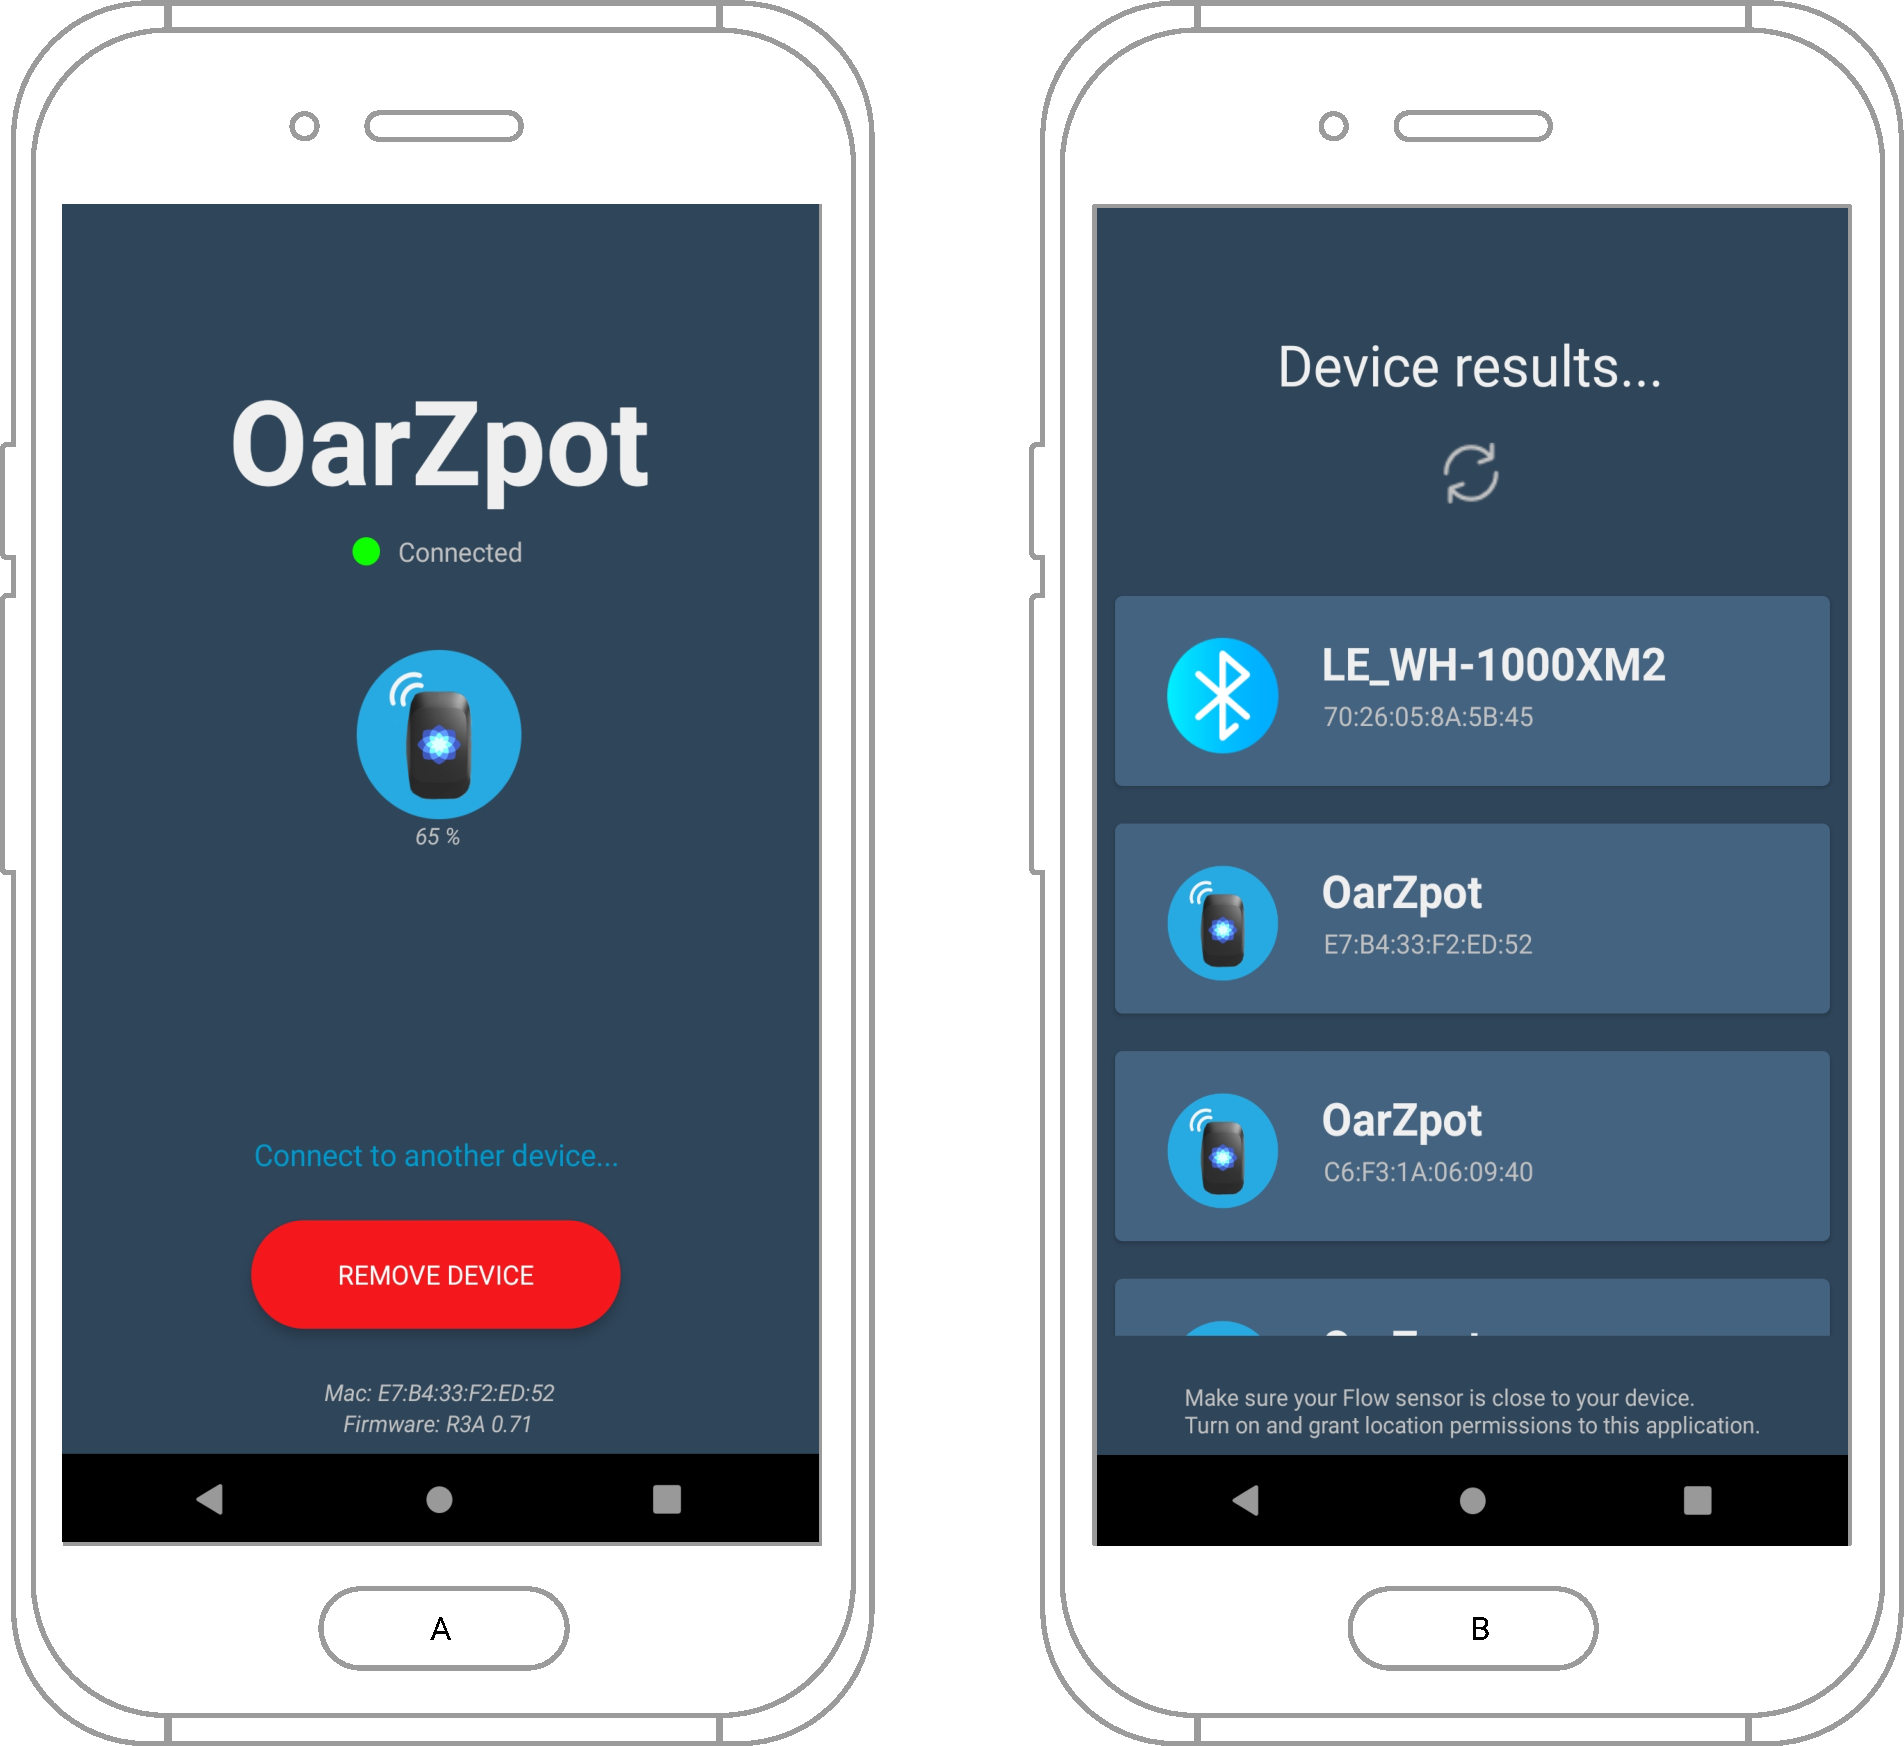
\includegraphics[scale=0.3]{images/flow_app.pdf}
    \caption{The Flow sensor wrapper screen to the user: (A) main screen, and (B) selecting a sensor source.}
    \label{fig:flowapp}
\end{figure}

\begin{itemize}
    \item[A] Is the main screen, that shows the state of the Flow sensor (e.g., battery level, MAC address, firmware version), including the button actions to either remove the sensor or change to another Flow sensor. 
    \item[B] In the cases, where there is no Flow sensor configured for the mobile device or the action to change the sensor, the device list screen display all available sensor or devices within range of BlueTooth connectivity to the user. The Flow sensors are distincitly from the other bluetooth devices, in order to make it easier to select.
\end{itemize}